\documentclass{beamer}
\usepackage{amsmath,graphics}
\usepackage{amssymb}

\usetheme{default}
\usepackage{xcolor}

\definecolor{solarizedBase03}{HTML}{002B36}
\definecolor{solarizedBase02}{HTML}{073642}
\definecolor{solarizedBase01}{HTML}{586e75}
\definecolor{solarizedBase00}{HTML}{657b83}
\definecolor{solarizedBase0}{HTML}{839496}
\definecolor{solarizedBase1}{HTML}{93a1a1}
\definecolor{solarizedBase2}{HTML}{EEE8D5}
\definecolor{solarizedBase3}{HTML}{FDF6E3}
\definecolor{solarizedYellow}{HTML}{B58900}
\definecolor{solarizedOrange}{HTML}{CB4B16}
\definecolor{solarizedRed}{HTML}{DC322F}
\definecolor{solarizedMagenta}{HTML}{D33682}
\definecolor{solarizedViolet}{HTML}{6C71C4}
%\definecolor{solarizedBlue}{HTML}{268BD2}
\definecolor{solarizedBlue}{HTML}{134676}
\definecolor{solarizedCyan}{HTML}{2AA198}
\definecolor{solarizedGreen}{HTML}{859900}
\definecolor{myBlue}{HTML}{162DB0}%{261CA4}
\setbeamercolor*{item}{fg=myBlue}
\setbeamercolor{normal text}{fg=solarizedBase03, bg=solarizedBase3}
\setbeamercolor{alerted text}{fg=myBlue}
\setbeamercolor{example text}{fg=myBlue, bg=solarizedBase3}
\setbeamercolor*{frametitle}{fg=solarizedRed}
\setbeamercolor*{title}{fg=solarizedRed}
\setbeamercolor{block title}{fg=myBlue, bg=solarizedBase3}
\setbeameroption{hide notes}
\setbeamertemplate{note page}[plain]
\beamertemplatenavigationsymbolsempty
\usefonttheme{professionalfonts}
\usefonttheme{serif}

\usepackage{fourier}

\def\vec#1{\mathchoice{\mbox{\boldmath$\displaystyle#1$}}
{\mbox{\boldmath$\textstyle#1$}}
{\mbox{\boldmath$\scriptstyle#1$}}
{\mbox{\boldmath$\scriptscriptstyle#1$}}}
\definecolor{OwnGrey}{rgb}{0.560,0.000,0.000} % #999999
\definecolor{OwnBlue}{rgb}{0.121,0.398,0.711} % #1f64b0
\definecolor{red4}{rgb}{0.5,0,0}
\definecolor{blue4}{rgb}{0,0,0.5}
\definecolor{Blue}{rgb}{0,0,0.66}
\definecolor{LightBlue}{rgb}{0.9,0.9,1}
\definecolor{Green}{rgb}{0,0.5,0}
\definecolor{LightGreen}{rgb}{0.9,1,0.9}
\definecolor{Red}{rgb}{0.9,0,0}
\definecolor{LightRed}{rgb}{1,0.9,0.9}
\definecolor{White}{gray}{1}
\definecolor{Black}{gray}{0}
\definecolor{LightGray}{gray}{0.8}
\definecolor{Orange}{rgb}{0.1,0.2,1}
\setbeamerfont{sidebar right}{size=\scriptsize}
\setbeamercolor{sidebar right}{fg=Black}

\renewcommand{\emph}[1]{{\textcolor{solarizedRed}{\itshape #1}}}

\newcommand\cA{\mathcal A}
\newcommand\cB{\mathcal B}
\newcommand\cC{\mathcal C}
\newcommand\cD{\mathcal D}
\newcommand\cE{\mathcal E}
\newcommand\cF{\mathcal F}
\newcommand\cG{\mathcal G}
\newcommand\cH{\mathcal H}
\newcommand\cI{\mathcal I}
\newcommand\cJ{\mathcal J}
\newcommand\cK{\mathcal K}
\newcommand\cL{\mathcal L}
\newcommand\cM{\mathcal M}
\newcommand\cN{\mathcal N}
\newcommand\cO{\mathcal O}
\newcommand\cP{\mathcal P}
\newcommand\cQ{\mathcal Q}
\newcommand\cR{\mathcal R}
\newcommand\cS{\mathcal S}
\newcommand\cT{\mathcal T}
\newcommand\cU{\mathcal U}
\newcommand\cV{\mathcal V}
\newcommand\cW{\mathcal W}
\newcommand\cX{\mathcal X}
\newcommand\cY{\mathcal Y}
\newcommand\cZ{\mathcal Z}

\newcommand\fA{\mathfrak A}
\newcommand\fB{\mathfrak B}
\newcommand\fC{\mathfrak C}
\newcommand\fD{\mathfrak D}
\newcommand\fE{\mathfrak E}
\newcommand\fF{\mathfrak F}
\newcommand\fG{\mathfrak G}
\newcommand\fH{\mathfrak H}
\newcommand\fI{\mathfrak I}
\newcommand\fJ{\mathfrak J}
\newcommand\fK{\mathfrak K}
\newcommand\fL{\mathfrak L}
\newcommand\fM{\mathfrak M}
\newcommand\fN{\mathfrak N}
\newcommand\fO{\mathfrak O}
\newcommand\fP{\mathfrak P}
\newcommand\fQ{\mathfrak Q}
\newcommand\fR{\mathfrak R}
\newcommand\fS{\mathfrak S}
\newcommand\fT{\mathfrak T}
\newcommand\fU{\mathfrak U}
\newcommand\fV{\mathfrak V}
\newcommand\fW{\mathfrak W}
\newcommand\fX{\mathfrak X}
\newcommand\fY{\mathfrak Y}
\newcommand\fZ{\mathfrak Z}

\newcommand\fa{\mathfrak a}
\newcommand\fb{\mathfrak b}
\newcommand\fc{\mathfrak c}
\newcommand\fd{\mathfrak d}
\newcommand\fe{\mathfrak e}
\newcommand\ff{\mathfrak f}
\newcommand\fg{\mathfrak g}
\newcommand\fh{\mathfrak h}
%\newcommand\fi{\mathfrak i}
\newcommand\fj{\mathfrak j}
\newcommand\fk{\mathfrak k}
\newcommand\fl{\mathfrak l}
\newcommand\fm{\mathfrak m}
\newcommand\fn{\mathfrak n}
\newcommand\fo{\mathfrak o}
\newcommand\fp{\mathfrak p}
\newcommand\fq{\mathfrak q}
\newcommand\fr{\mathfrak r}
\newcommand\fs{\mathfrak s}
\newcommand\ft{\mathfrak t}
\newcommand\fu{\mathfrak u}
\newcommand\fv{\mathfrak v}
\newcommand\fw{\mathfrak w}
\newcommand\fx{\mathfrak x}
\newcommand\fy{\mathfrak y}
\newcommand\fz{\mathfrak z}

\newcommand\vA{\vec A}
\newcommand\vB{\vec B}
\newcommand\vC{\vec C}
\newcommand\vD{\vec D}
\newcommand\vE{\vec E}
\newcommand\vF{\vec F}
\newcommand\vG{\vec G}
\newcommand\vH{\vec H}
\newcommand\vI{\vec I}
\newcommand\vJ{\vec J}
\newcommand\vK{\vec K}
\newcommand\vL{\vec L}
\newcommand\vM{\vec M}
\newcommand\vN{\vec N}
\newcommand\vO{\vec O}
\newcommand\vP{\vec P}
\newcommand\vQ{\vec Q}
\newcommand\vR{\vec R}
\newcommand\vS{\vec S}
\newcommand\vT{\vec T}
\newcommand\vU{\vec U}
\newcommand\vV{\vec V}
\newcommand\vW{\vec W}
\newcommand\vX{\vec X}
\newcommand\vY{\vec Y}
\newcommand\vZ{\vec Z}

\newcommand\va{\vec a}
\newcommand\vb{\vec b}
\newcommand\vc{\vec c}
\newcommand\vd{\vec d}
\newcommand\ve{\vec e}
\newcommand\vf{\vec f}
\newcommand\vg{\vec g}
\newcommand\vh{\vec h}
\newcommand\vi{\vec i}
\newcommand\vj{\vec j}
\newcommand\vk{\vec k}
\newcommand\vl{\vec l}
\newcommand\vm{\vec m}
\newcommand\vn{\vec n}
\newcommand\vo{\vec o}
\newcommand\vp{\vec p}
\newcommand\vq{\vec q}
\newcommand\vr{\vec r}
\newcommand\vs{\vec s}
\newcommand\vt{\vec t}
\newcommand\vu{\vec u}
\newcommand\vv{\vec v}
\newcommand\vw{\vec w}
\newcommand\vx{\vec x}
\newcommand\vy{\vec y}
\newcommand\vz{\vec z}

\renewcommand\AA{\mathbb A}
\newcommand\NN{\mathbb N}
\newcommand\ZZ{\mathbb Z}
\newcommand\PP{\mathbb P}
\newcommand\QQ{\mathbb Q}
\newcommand\RR{\mathbb R}
\renewcommand\SS{\mathbb S}
\newcommand\CC{\mathbb C}

\newcommand{\ord}{\mathrm{ord}}
\newcommand{\id}{\mathrm{id}}
\newcommand{\pr}{\mathrm{P}}
\newcommand{\Vol}{\mathrm{vol}}
\newcommand\norm[1]{\left\|{#1}\right\|} 
\newcommand\sign{\mathrm{sign}}
\newcommand{\eps}{\varepsilon}
\newcommand{\abs}[1]{\left|#1\right|}
\newcommand\bc[1]{\left({#1}\right)} 
\newcommand\cbc[1]{\left\{{#1}\right\}} 
\newcommand\bcfr[2]{\bc{\frac{#1}{#2}}} 
\newcommand{\bck}[1]{\left\langle{#1}\right\rangle} 
\newcommand\brk[1]{\left\lbrack{#1}\right\rbrack} 
\newcommand\scal[2]{\bck{{#1},{#2}}} 
\newcommand{\vecone}{\mathbb{1}}
\newcommand{\tensor}{\otimes}
\newcommand{\diag}{\mathrm{diag}}
\newcommand{\ggt}{\mathrm{ggT}}
\newcommand{\kgv}{\mathrm{kgV}}
\newcommand{\trans}{\top}

\newcommand{\Karonski}{Karo\'nski}
\newcommand{\Erdos}{Erd\H{o}s}
\newcommand{\Renyi}{R\'enyi}
\newcommand{\Lovasz}{Lov\'asz}
\newcommand{\Juhasz}{Juh\'asz}
\newcommand{\Bollobas}{Bollob\'as}
\newcommand{\Furedi}{F\"uredi}
\newcommand{\Komlos}{Koml\'os}
\newcommand{\Luczak}{\L uczak}
\newcommand{\Kucera}{Ku\v{c}era}
\newcommand{\Szemeredi}{Szemer\'edi}

\renewcommand{\ae}{\"a}
\renewcommand{\oe}{\"o}
\newcommand{\ue}{\"u}
\newcommand{\Ae}{\"A}
\newcommand{\Oe}{\"O}
\newcommand{\Ue}{\"U}

\newcommand{\im}{\mathrm{im}}
\newcommand{\rrk}{\mathrm{zrg}}
\newcommand{\crk}{\mathrm{srg}}
\newcommand{\rk}{\mathrm{rg}}
\newcommand{\GL}{\mathrm{GL}}
\newcommand{\SL}{\mathrm{SL}}
\newcommand{\SO}{\mathrm{SO}}
\newcommand{\nul}{\mathrm{nul}}
\newcommand{\eig}{\mathrm{eig}}

\newcommand{\mytitle}{Clustering}

\title[Linadi]{\mytitle}
\author[Amin Coja-Oghlan]{Amin Coja-Oghlan}
\institute[Frankfurt]{JWGUFFM}
\date{}

\begin{document}

\frame[plain]{\titlepage}

\begin{frame}\frametitle{\mytitle}
	\begin{block}{Inhalt}
		\begin{itemize}
			\item Wir lernen eine Anwendung der Linearen Algebra kennen.
			\item Es geht um einen Algorithmus, der Cluster in einem Netzwerk erkennt.
			\item Ein Cluster ist dabei eine Menge von Netzwerkknoten, die ein wenig dichter verbunden sind als das Netzwerk ingesamt.
			\item \emph{Frage:} wie k\oe nnen wir die Clusterstruktur eines Netzwerkes ``lernen''?
		\end{itemize}
	\end{block}
\end{frame}

\begin{frame}\frametitle{\mytitle}
	\hfill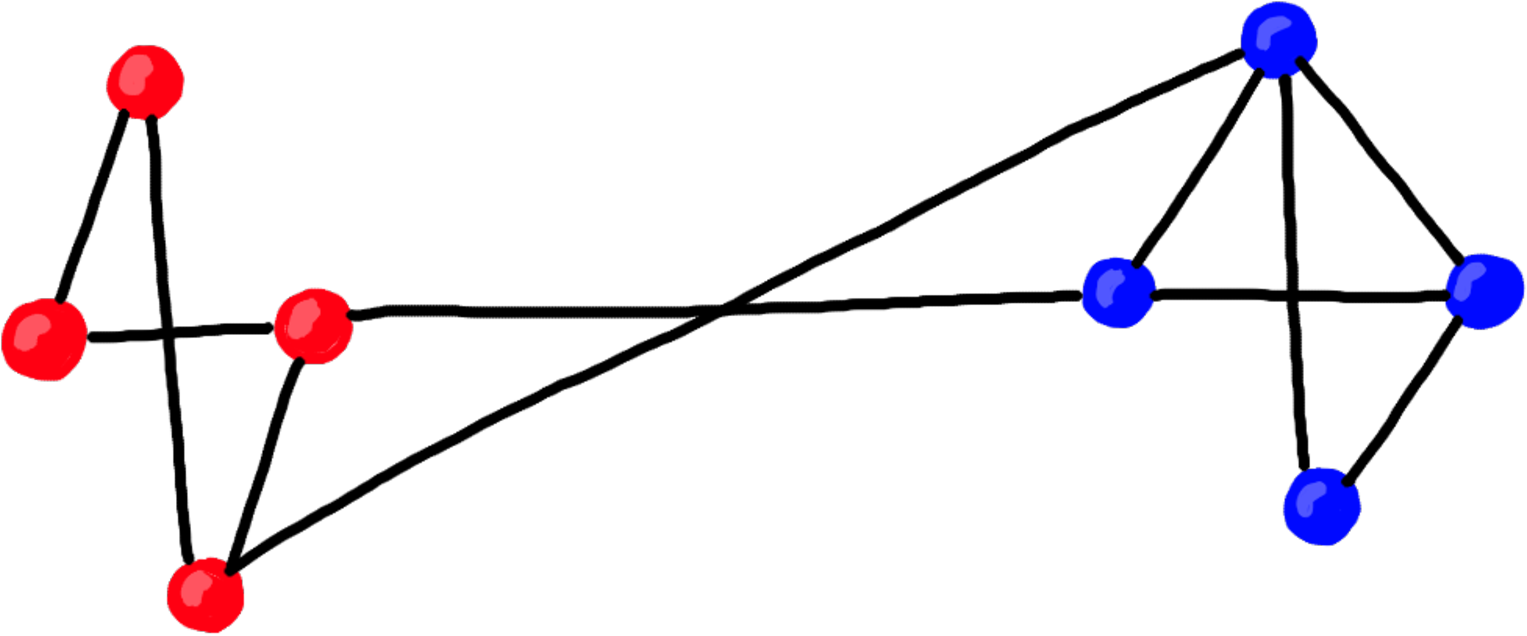
\includegraphics[height=20mm]{pics/sbm.pdf}
	\begin{block}{Ein Zufallsmodell}
		\begin{itemize}
			\item Um das Problem zu modellieren, betrachten wir einen zuf\ae llig erzeugten Graphen.
			\item Der Graph hat $n$ Knoten f\ue r eine gerade Zahl $n$.
			\item Wir sie in zwei gleichgro\ss e zuf\ae llige Teilmengen $V_1,V_2$ auf.
			\item Je zwei Knoten in derselben Klasse sind mit Wahrscheinlichkeit $p$ verbunden.
			\item Knoten in unterschiedlichen Klassen sind mit Wahrscheinlichkeit $q<p$ verbunden.
			\item Alle Verbindungen sind unabh\ae ngig.
		\end{itemize}
	\end{block}
\end{frame}

\begin{frame}\frametitle{\mytitle}
	\hfill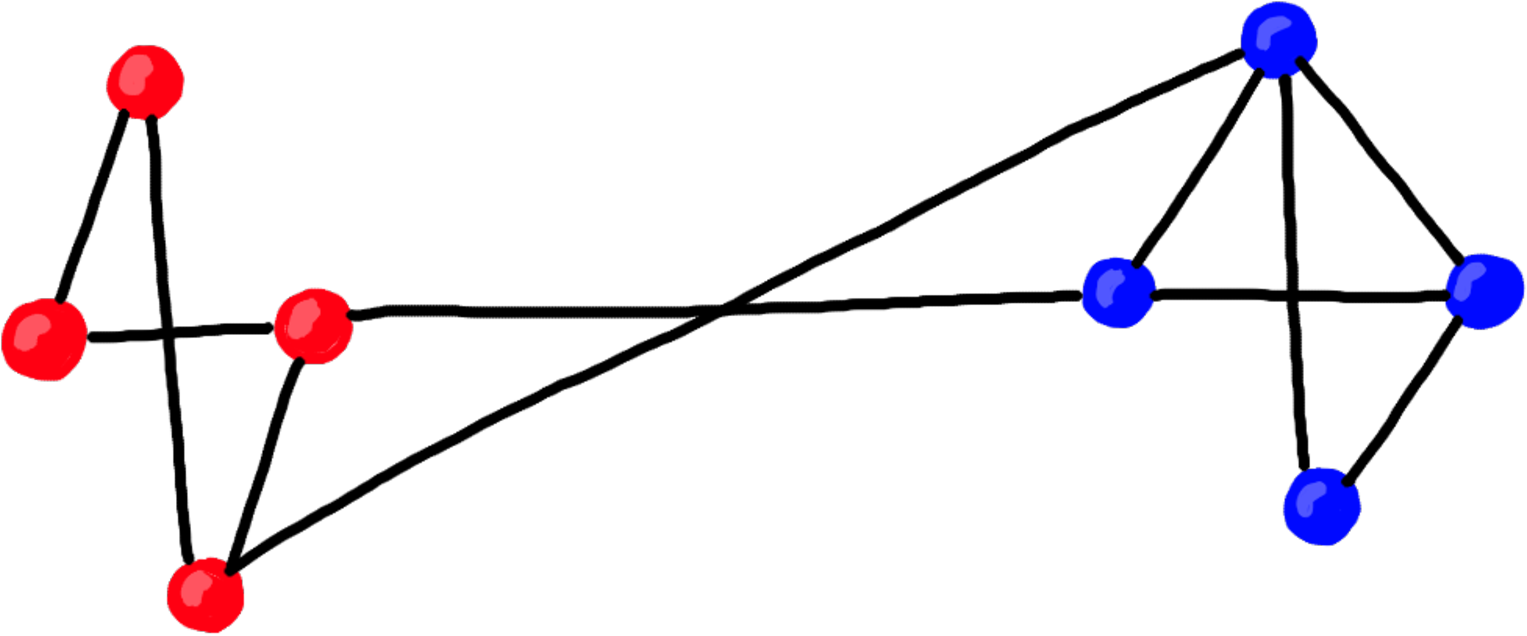
\includegraphics[height=20mm]{pics/sbm.pdf}
	\begin{block}{Ein Zufallsmodell}
		\begin{itemize}
			\item \emph{Frage:} gegeben den Graphen $G$, k\oe nnen wir $V_1,V_2$ rekonstruieren?
			\item Die Antwort wird von $n,p,q$ abh\ae ngen.
			\item Je gr\oe\ss er $n$, desto mehr Information haben wir.
			\item Je gr\oe\ss er $p-q$, desto klarer treten $V_1,V_2$ hervor.
		\end{itemize}
	\end{block}
\end{frame}

\begin{frame}\frametitle{\mytitle}
	\begin{block}{Naiver Algoritmus}
		\begin{itemize}
			\item Wir k\oe nnten alle m\oe glichen Mengen $V_1,V_2$ durchprobieren.
			\item Die `richtige' L\oe sung k\oe nnte die Zerlegung mit den meisten Kanten innerhalb der Cluster sein.
			\item Allerdings gibt es $2^n$ M\oe glichkeiten.
			\item Selbst f\ue r kleine Werte wie $n=100$ dauert das zu lange.
		\end{itemize}
	\end{block}
\end{frame}

\begin{frame}\frametitle{\mytitle}
	\begin{block}{Die Adjazenzmatrix}
		\begin{itemize}
			\item Der Graph $G$ induziert eine Matrix $A=A(G)=(a_{ij})_{i,j=1,\ldots,n}$ mit Eintr\ae gen
				\begin{align*}
					a_{ij}&=\begin{cases}1&\mbox{ falls }v_i,v_j\mbox{ verbunden sind}\\0&\mbox{ sonst}\end{cases}
				\end{align*}
			\item Wir nennen $A$ die \emph{Adjazenzmatrix} von $G$.
			\item Sie ist symmetrisch.
			\item Weil $G$ zuf\ae llig ist, ist $A$ eine zuf\ae llige Matrix.
		\end{itemize}
	\end{block}
\end{frame}

\begin{frame}\frametitle{\mytitle}
	\begin{block}{Heuristik: Approximation von geringem Rang}
		\begin{itemize}
			\item betrachte die $n\times n$-Matrix $B$ mit Eintr\ae gen
				\begin{align*}
					b_{ij}&=\begin{cases}p&\mbox{ falls $v_i,v_j\in V_1$ oder $v_i,v_j\in V_2$}\\q&\mbox{ sonst}.\end{cases}
				\end{align*}
			\item wenn $V_1=\{v_1,\ldots,v_{n/2}\}$ und $V_2=\{v_{n/2+1},\ldots,v_n\}$ hat $B$ die Form
				\begin{align*}
					B&=\begin{pmatrix}
						p&\cdots&p&q&\cdots&q\\
						\vdots&\ddots&\vdots&\vdots&\ddots&\vdots\\
						p&\cdots&p&q&\cdots&q\\
						q&\cdots&q&p&\cdots&p\\
						\vdots&\ddots&\vdots&\vdots&\ddots&\vdots\\
						q&\cdots&q&p&\cdots&p
					\end{pmatrix}
				\end{align*}
		\end{itemize}
	\end{block}
\end{frame}

\begin{frame}\frametitle{\mytitle}
	\begin{block}{Heuristik: Approximation von geringem Rang}
		\begin{itemize}
			\item die Matrix $B$ hat Rang $2$
			\item die Eigenwerte sind $n(p+q)/2$ mit Eigenvektor $\vecone$, und
			\item $n(p-q)/2$ mit Eigenvektor $(1,\ldots,1,-1,\ldots,-1)^\trans$.
			\item An dem zweiten Eigenvektor kann man $V_1,V_2$ ablesen!
		\end{itemize}
	\end{block}
\end{frame}

\begin{frame}\frametitle{\mytitle}
	\begin{block}{Heuristik: Approximation von geringem Rang}
		\begin{itemize}
			\item wir k\oe nnen noch den Eigenvektor $\vecone$ ``ausblenden''.
			\item dazu ziehen wir $(p+q)/2$ von jedem Matrixeintrag ab:
				\begin{align*}
					C&=\frac{1}{2}	
\begin{pmatrix}
						p-q&\cdots&p-q&q-p&\cdots&q-p\\
						\vdots&\ddots&\vdots&\vdots&\ddots&\vdots\\
						p-q&\cdots&p-q&q-p&\cdots&q-p\\
						q-p&\cdots&q-p&p-q&\cdots&p-q\\
						\vdots&\ddots&\vdots&\vdots&\ddots&\vdots\\
						q-p&\cdots&q-p&p-q&\cdots&p-q
					\end{pmatrix}
				\end{align*}
			\item Diese Matrix hat Rang $1$.
			\item Der Eigenvektor $(1,\ldots,1,-1,\ldots,-1)$ mit Eigenwert $n(p-q)/2$ ist erhalten geblieben.
		\end{itemize}
	\end{block}
\end{frame}

\begin{frame}\frametitle{\mytitle}
	\begin{block}{Heuristik: Approximation von geringem Rang}
		\begin{itemize}
			\item \emph{Heuristische Annahme:} schreibe $A=B+R$, wobei $R$ ein zuf\ae lliger ``Fehlerterm'' ist.
			\item Vielleicht ist $R$ ``klein'' genug, so da\ss\ $(1,\ldots,1,-1,\ldots,-1)$ immer noch ungef\ae hr Eigenvektor von $A$ ist.
			\item Dann k\oe nnten wir einfach dominanten Eigenvektor $y$ von
				\begin{align*}
					M=A-\frac{p+q}{2}\vecone
				\end{align*}
				berechnen.
			\item Unsere Sch\ae tzung der Partition $V_1,V_2$ w\ae re dann
				\begin{align*}
					V_1'&=\cbc{v_i:y_i\geq0}&V_2&=\cbc{v_i:y_i<0}.
				\end{align*}
		\end{itemize}
	\end{block}
\end{frame}

\begin{frame}\frametitle{\mytitle}
	\begin{block}{Berechnung des Eigenvektors}
		\begin{itemize}
			\item Wie berechnen wir den Eigenvektor $y$?
			\item \emph{Idee:} erzeuge einen zuf\ae lligen Vektor $s$.
			\item Sei $u_1,\ldots,u_n$ eine Orthonormalbasis aus Eigenvektoren von $M$, mit Eigenwerten $\lambda_1\geq\ldots\geq\lambda_n$.
			\item Wir zerlegen $s$ in der Form
				\begin{align*}
					s&=\sum_{i=1}^n t_iu_i.
				\end{align*}
			\item Dann gilt
				\begin{align*}
					Ms&=\sum_{i=1}^n\lambda_it_iu_i.
				\end{align*}
		\end{itemize}
	\end{block}
\end{frame}

\begin{frame}\frametitle{\mytitle}
	\begin{block}{Berechnung des Eigenvektors}
		\begin{itemize}
			\item Allgemeiner erhalten wir f\ue r $\ell\in\NN$:
				\begin{align*}
					M^\ell s&=\sum_{i=1}^n\lambda_i^\ell t_iu_i.
				\end{align*}
			\item Wenn jetzt $\lambda_1$ deutlich gr\oe\ss er ist als die \ue brigen $\lambda_i$, gilt f\ue r hinreichend gro\ss e $\ell$ die Approximation
				\begin{align*}
				M^\ell s\approx\lambda_1^\ell t_i u_i.
				\end{align*}
			\item Mit $z=M^\ell s$ k\oe nnen wir also die Cluster approximieren durch
\begin{align*}
					V_1'&=\cbc{v_i:z_i\geq0}&V_2&=\cbc{v_i:z_i<0}.
				\end{align*}
		\end{itemize}
	\end{block}
\end{frame}

\begin{frame}\frametitle{\mytitle}
	\begin{block}{Zusammenfassung}
		\begin{itemize}
			\item Wir haben als Anwendung der Linearen Algebra in der Informatik ein Clusteringproblem untersucht.
			\item Eigenvektorberechnungen k\oe nnen benutzt werden, um Clusteringprobleme heuristische zu l\oe sen.
			\item Dies f\ue hrt zu effizienten Verfahren f\ue r scheinbar schwierige Probleme.
		\end{itemize}
	\end{block}
\end{frame}
\end{document}
